\chapter{Cibles de fonctionnement}


\section{Axes d'amélioration}

    Les chapitres précédents --- analyse de l'existant et benchmarking -- permettent d'identifier quelques axes sur lesquels le système d'information de SPIE péche contre les bonnes pratiques et où des améliorations sont à prévoir.

    Nous allons donc citer dans ce document certains thèmes d'amélioration possibles à travers les axes suivant:

    \begin{enumerate}
        \item Identification de nouvelles technologies à forte valeur ajoutée~;
        \item Réorganisation des acteurs des processus métiers de SPIE pour suivre les ``best-practices'' dégagées~;
        \item Réorganisation de la logique des processus existants~;
    \end{enumerate}


    \subsection{Nouvelles technologies}

    L'intégration de nouvelles technologies peut permettre à SPIE de se démarquer de la concurrence en changeant de manière radicale la gestion de certaines opérations.

    Nous allons nous intéresser à certaines technologies que SPIE pourrait intégrer~:

        \subsubsection{Gestion de la Relation Client avec un CRM}

        Quand on s'intéresse à la cartographie générale du SI de SPIE, la première chose qu'on remarque est l'absence d'une gestion de la Relation Client en utilisant un outil dédié, de type CRM.

        Les outils CRM (\textit{Customer Relationship Management}, ou Gestion de la Relation Client) permettent une gestion optimale la Relation Client avec des outils de modélisation, de reporting et de prédiction.

        L'utilisation d'outils dédiés permet autant d'améliorer les processus de Relation Client que de prédire les attentes de clients et ainsi prévenir les échecs et mieux s'y préparer. Là où SPIE utilise actuellement plusieurs outils (\texit{Clarify}, \textit{ADV}, \textit{SUPRA}) aux infrastructures parfois séparées, l'utilisation d'un seul CRM simplifierai les processus de facturation, de suivi contrats et autres processus clients, et permettrait une meilleure intégration entre ces derniers.

        Les outils CRM permettent en outre de mener des campagnes de prospection, de suivre les opportunités commerciales et de fidéliser les clients.

        On peut citer à titre d'exemple \textit{Salesforce}, l'un des leaders du marché qui propose un CRM en mode \textit{SaaS}.


    % TODO : donner + de nouvelles technologies et notamment parler de ça :
    %
    % * Donner aux techniciens un appareil qui permet de reporter les applications faites sur place
    % * Affecter un (ou des) techniciens à chaque client. Le technicien connaîtra déjà l'infrastructure du client à chaque intervention ce qui devrait accélérer les choses et donner un meilleur processus


\section{Les attentes client}

	Les clients ont certaines attentes lorsqu'ils signent un contrat (qui varient selon le client). Ci dessous nous allons lister les plus importantes d'entre elles qui peuvent apparaître.

\begin{itemize}
	\item une certaine proximité (couvrir le territoire)~;
	\item un support technologique~;
	\item de l'innovation~;
	\item de l'expertise~;

	\item assurer la gestion contractuelle et le reporting~;
	\item gérer les interventions (intervention forfaitaire : préventive et curative standard ; intervention en bon de commande : curative exceptionnelle, amélioration installations, traitement obsolescence...)~;
	\item une identification des risques techniques, financiers et organisationnels~;
	\item un compte rendu de l'état des lieux initial (pour les soldes d'écart si des travaux en plus sont nécessaires~;

	\item une améliorer le cadre de vie~;
	\item un respecter l'environnement~;

	\item un accompagnement dans la conception, la réalisation, l'exploitation et la maintenance~; d'installations plus économes en énergie et plus respectueuse de l'environnement~;
	\item un suivi des spécifications du client~;
	\item un suivi des avancements pour le client~;
	\item une construction et validation des processus avec le client~;
	\item une revue périodique du contrat pour les décisions à renouveler ou non, et la prise en compte de réclamations du client~;
	\item des preuves du respect des engagements (bonne mise en œuvre, et adaptation au besoin).
\end{itemize}


\section{Les nouvelles règles de gestion}
Dans cette partie, nous allons proposer certaines règles standard qui pourront aider à réduire les dysfonctionnements dans la gestion des contrats de maintenance.


\section{Processus Retour d'exéprience}

\begin{figure}[h!]
	\centering
	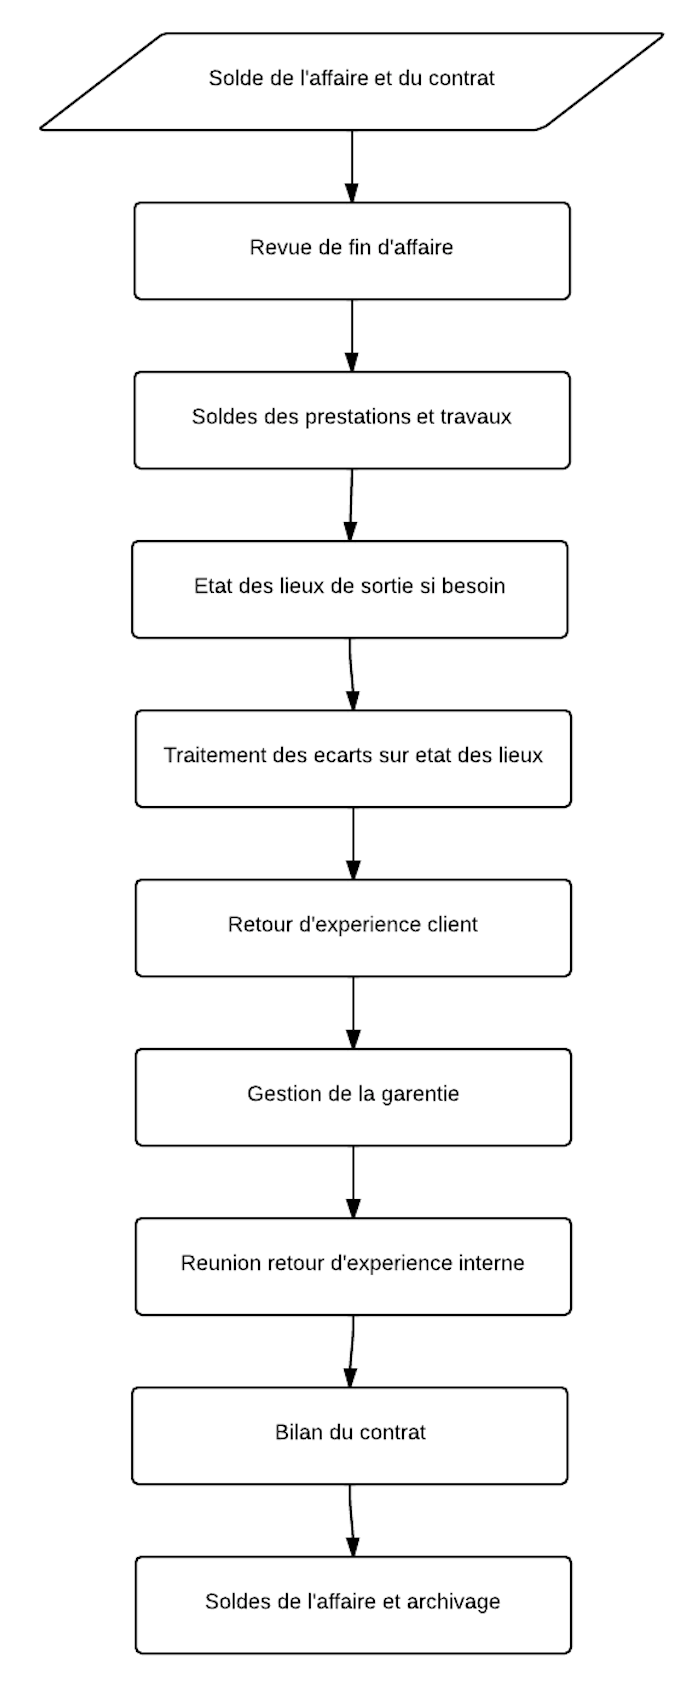
\includegraphics[width=0.45\linewidth]{images/processus_retour_experience.png}
	\caption{Processus de retour d’expérience}
	\label{fig:processusRetourExperience}
\end{figure}

Ainsi l'ajout du processus \textit{retour d'\'exp\'erience client} dans le sous-processus \textit{solde
de l'affaire et du contrat} r\'epond aux exigences de SPIE Sud Est suivante~:

\begin{itemize}
    \item Base de connaissance m\'etier type de contrat~;
    \item Identification des risques techniques/financiers/organisationnels.
\end{itemize}

